\chapter{Methodology}

This research is geared towards finding a correlation between users' biometric data to their performance in a first-person shooter gaming scenario. The quality of the user data 
collected was critical in ensuring that the research aims were achieved. For Quality Assurance purposes, a systematic step-by-step approach has been designed for the data-capturing 
process. An activity monitoring device was distributed to the volunteers in the form of a Polar Watch. The individuals were instructed to use these devices at pre-designated times 
prior to undertaking a test in the form of a First-Person Shooter Game. Results from the test, was than paired with their biometric data for further analysis.

\section{Requirements Engineering}
The requirements engineering process was carried focusing on the research objectives. It was divided into the following stages:

\subsection{Requirement Input}
The research objectives were determined by the client. The research objectives were to find a correlation between users' biometric data to their performance in a
first-person shooter gaming scenario. The research objectives were used as the input for the requirements engineering process.

\subsection{Requirement Analysis}
The feasibility study was carried out to determine the resources that would be required to implement the research objectives and to determine the time frame for the research. 

\subsection{Requirement Specification}
After analyzing the requirements, the final specifications were defined for the research. The final specifications were used as the input for the design process.

\section{Analysis}
The analysis phase involved examining the collected biometric data and gaming performance results to identify patterns and correlations. The analysis was carried 
out in the following stages:

\subsection{Recruitment of Volunteers}
The process of recruiting the volunteers was carried out in a way that ensured they satisfied the conditions of the research. The volunteers were required to be students of the Atlantic 
Technological University (ATU) Galway campus. The volunteers were also required to be over the age of 18 and have no known medical conditions that could affect their performance in the
test. A Microsoft form was created and distributed to the students of the university to register their interest in the research. A poster \ref{fig:recruitment-poster} was created
which contained information about the research and a QR code that linked to the Microsoft form.

\begin{figure}[ht]
    \centering
    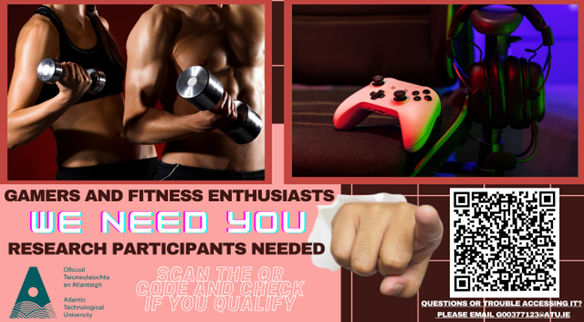
\includegraphics[width=0.95\linewidth]{images/poster.png}
    \caption{Volunteers Recruitment Poster}
    \label{fig:recruitment-poster}
\end{figure}

The form can be found in the appendix \ref{sec:form-recruitment}.
For a volunteer to be considered, they were required to fill out the form and submit it. The form was designed to capture the following information from the volunteers:

\begin{itemize}
    \item How often the participant practices exercises.
    \item The average duration of the exercises sessions.
    \item If the participant owns a activity monitoring device, if so which brand (Polar, Garmin, Apple, FitBit, or other).
    \item If the participant plays video games, if so which platform (PC, Xbox, Playstation, or other).
    \item Which game genre the participant enjoy the most. (First Person Shooter, Third Person Shooter, Soccer, Car Racing, or other).
    \item Participant should also sign the form as a consent to participate in the research.
\end{itemize}

\subsection{Data Collection}

For the purpose of the research, different categories of data was collected from the volunteers through the monitoring device to help achieve the stated goals. As personal data was
being collected, an application to the Ethics Research and Ethics Committee was made to ensure that the data collection process was in compliance with the General Data Protection.

\par 
The Taught Programme Research Ethics Approval Application Form can be found on appendix \ref{sec:ethics-application}. It was an extensive and iterative process with the Ethics Research and Ethics 
office to ensure that the data collection process was in compliance with the General Data Protection Regulation (GDPR). Unfortunately, it took longer than expected to get the approval
from the Ethics Research and Ethics Committee, which lead to an unexpected delay in the data collection process. The data collection process was divided into two main categories:

\subsubsection*{Biometric Data}

For the very first time processing a volunteer, some user information was needed to have them registered with the activity monitoring device and their data was saved to the manufacturer'
repository. The Activity Monitoring Device used on this research was the Polar Vantage Smart Watch. The watch is capable of monitoring and capturing user’s biometric data and saving the
data to a repository where it can be accessed online via an API. The device is commercially available and accessible to the public. The rationale for using the Polar Vantage Watch is
that it has been widely used in both academic and industrial research projects and validation. Most importantly, these devices were available to us in such quantity that could satisfy
our research needs.

\subsubsection*{Physical Information}

The following physical information was collected from the volunteers, and stored with the manufacturer (Polar) which is GDPR compliant. The data was then accessed through the Polar API.

\begin{itemize}
    \item Sleep Data: According to the manufacturer's manual \cite{polarManual}, the watch can record both the quality and quantity of sleep, providing insights into
    the duration spent on the stages of sleep, such as REM Sleep, Deep Sleep and Light Sleep, Deep Sleep, and REM Sleep, along with the respective durations of each sleep stage. For the purpose of the research, an aggregated total of the various categories of sleep was 
    recorded and used.
    Volunteers were instructed to wear the watch to sleep on the previous night before their scheduled test. Unit of measure used for the sleep data is minutes. 
    \item Daily Activities: According to the Activity monitor manufacturers' manual \cite{polarManual}, "Polar device uses an internal 3D accelerometer to record the wrist movements. It analyses the frequency, 
    intensity and regularity of the movements together with the physical information." Calories, active calories, active steps and their respective durations are collected from through the device. For the 
    purpose of the research, the active steps was used. Volunteers were expected to wear the device on the previous day for this data to be available. Unit of measure used for the daily activities is count of steps.
    \item Nightly Recharge: From the Activity monitor manufacturers' manual \cite{polarManual}, the Nightly Recharge is recorded as follows: " is an overnight recovery measurement that shows how well your body has
    coped with overall stress you have experienced lately." The parameters, measured during roughly the first four hours of your sleep are heart rate, heart rate variability and breathing rate. For the purpose 
    of the research, the following parameters and derived parameters was used:
    \begin{itemize}
        \item Heart Rate Average (bpm)
        \item Heart Rate Maximum (bpm)
        \item Heart Rate Variability (HRV)
    \end{itemize}
\end{itemize}

\subsubsection*{Test Data Collection}
The test data is generated at the completion of the test session in the Unit Test Application. A test session consists of three categories of tests, which is undertaken sequentially in different stages. 
For quality assurance, the test was performed in a controlled environment using the same hardware in similar conditions over the course of the trials. For the purpose of the trial, a special designated room
has been reserved for the data collection effort. The following metrics for the different tests was then captured and subsequently used for the research effort.

\begin{itemize}
    \item Audio Test: designed to test users’ audio reflexes. 
    \item Audio Average Response Time: this is a measure of how quickly a user is able to react and determine the origin of a sound based on the audibility variance (in decibels) in a 3-Dimensional space. 
    \item Visual Test: designed to test users’ visual perception. At the end of this category of test, the following metrics were designed to measure users’ performance. 
    \item Visual Average Response Time: a measure of how quickly a user can identify and engage targets. 
    \item Shot Accuracy: a measure of the percentage of successful shots to the number of targets spawned. 
    \item Target Accuracy: a measure of the percentage of successful shots taken to a number of targets hit. 
    \item Fine Motor Test: designed to test users’ perception of depth and eye to hand coordination. 
    \item Average Tracking Time: measure of average time it took for a player to successfully track, engage, and eliminate a target.
    \item Accuracy: measure of the percentage of shots fired to the number of targets hit. 
\end{itemize}

\subsubsection{Data Collection Procedure}

The data collection process followed the below-listed steps to maximize throughput and minimize the average time spent processing each participant. The whole procedure can be found in the appendix \ref{appendix}.
\par
For this study, participants were required to wear the Polar watch which is referred sometimes as “Activity Monitoring Device” in this text, a day prior to undertaking a gaming test. 

\subsubsection*{Location:}

The data collection effort was carried out at the Gym on the Atlantic Technological University (ATU) Galway campus.

\subsubsection*{Time:}

The following weekly schedule was available for the volunteers at various times that best suit their personal schedules.
\begin{itemize}
    \item Tuesdays: 12:00 - 13:00, 15:00 - 16:00
    \item Wednesdays: 12:00 - 13:00, 15:00 - 16:00
    \item Thursdays: 12:00 - 13:00, 15:00 - 16:00
    \item Fridays: 13:00 - 15:00
\end{itemize}

Results of the test were then paired with their biometric data for further analysis.

\section{Design and Development}

As a software development methodology for this project, many factors were considered. Initially, a comparison of the different software development methodologies was carried out to determine
which would be the most suitable for the project. The comparison was based on the following factors:

\begin{itemize}
    \item Continuous Stakeholder Involvement: The methodology should allow for continuous stakeholder involvement in the development process. Maintaining a continuous feedback loop with the 
    stakeholders was essential for the project. 
    \item Flexibility in Requirements: The methodology should allow for flexibility in the requirements. The requirements were not completely established at the start. The methodology should allow for changes to be made to the requirements as the project progresses.
    \item Iterative Development: The methodology should allow for iterative development. As the project was divided into different phases, each phase should be developed iteratively, allowing for the project to be developed in a series of small, manageable steps.    
\end{itemize}

After all the considerations, Agile Methodology \cite{despa2014comparative} appeared as the preferred choice over Waterfall, as it allows for continuous stakeholder involvement, flexibility in requirements and iterative development.
Unlike the rigid Waterfall methodology \cite{despa2014comparative}, Agile allows for changes to be made to the requirements as the project progresses. The Agile methodology also allows for the project to be developed in a series of small, manageable steps.
This iterative nature enabled continuous refinement and adjustment, ensuring that the stakeholders were satisfied with the progress.

\subsubsection*{Agile - Extreme Programming (XP)}
Extreme Programming (XP) is an Agile framework that moves from the traditional software development methodologies by breaking down the development process into smaller and more manageable increments.
Instead of extensive planning, analysis, and design upfront, XP focuses on continuous and iterative development. To minimize errors and defects, XP places a strong emphasis on testing.
This test-driven development approach ensures that the code is always working and that any defects are caught early in the development process.
XP also places a strong emphasis on customer satisfaction. The customer is involved in the development process and is able to provide feedback on the project as it progresses. \cite{despa2014comparative} 
In general, Extreme Programming presents a flexible and iterative method for software development that aligns well with the requirements of this project.

\begin{figure}
    \centering
    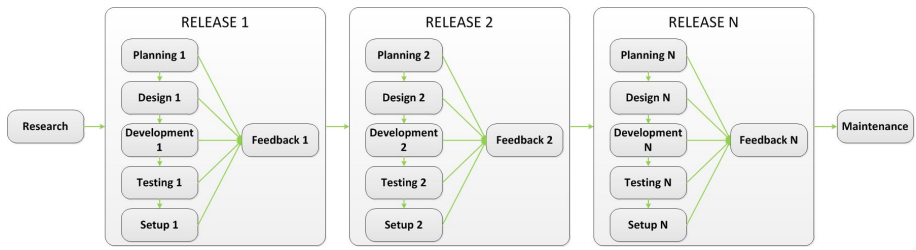
\includegraphics[width=1.0\linewidth]{images/xp.png}
    \caption{Extreme programming methodology \cite{despa2014comparative}}
    \label{fig:agile}
\end{figure}

Figure \ref{fig:agile} shows the Extreme Programming methodology. The methodology is divided into four main phases: Planning, Designing, Coding, and Testing. 
Each phase is developed iteratively, allowing for the project to be developed in a series of small, manageable steps. 

\subsection{Testing}
As part of testing the system, the following steps were taken to ensure that the system met the stakeholders' requirements:

\begin{itemize}
    \item Mocha Testing: this test was carried out to ensure that the API endpoints were working correctly and that the data was being retrieved correctly.
    \item Integration Testing: this test was responsible for testing how the different components of the system worked together.
    \item System Testing: this test was carried out to ensure that the entire system worked as expected and that it met the stakeholders' requirements.
\end{itemize}
    

\subsection{Deployment}

After the system was accepted by the stakeholders, it was deployed to the server where it could be accessed. 

\subsection{Maintenance and Update}

Following deployment, the system was maintained and updated as needed to ensure that it continued to meet the stakeholders' requirements. Regular updates
were made to the system to ensure that it remained up-to-date and that it continued to meet the stakeholders' needs.

\section{Meetings}
In this section we will discuss the different types of meetings that were held throughout the project. The meetings were held to ensure that the project was on track
and that the stakeholders were satisfied with the progress.

\subsection{Supervisor Meetings}
Weekly meeting was setup with the supervisor to discuss the progress of the project. The meetings were held in the supervisor's office on campus every Tuesday at 12 pm throughout
the duration of the project. The meetings were used to discuss:

\begin{itemize}
    \item The progress of the project.
    \item Any issues or challenges that were encountered.
    \item Any changes that needed to be made to the project.
    \item Any feedback that the supervisor had on the project.
\end{itemize}

These meetings were important, especially in the early stages of the project, due to various challenges that were encountered. The feedback from the supervisor was invaluable
in helping to overcome these challenges.

\subsection{Client Meetings}

At the beginning of the year we were offered the opportunity to work with a client on a project. In our meeting with the client, we were informed that the project
was a research project that aimed to find a correlation between users' biometric data to their performance in a first-person shooter gaming scenario. The aim was to quantify
how biometric such as Heart Rate Variation, Heart Rate, active steps taken, quality and quantity of sleep, etc. affect select gaming skills like eye-to-hand coordination, fine-motor skills and reaction time.
The client also informed us that the project was a continuation of a previous project and that we would be inheriting an existing infrastructure. 
For the collection of the biometric data, the client informed us that there was four Polar Vantage Smart Watches available for the project. The meetings were also held to get
the devices registered on the Polar API and to get the volunteers enrolled in the project. 

The meetings were held online using Teams and also in the client's office in the ATU Gym at Unit D, Racecourse Business Park, Ballybrit, Galway. 

\section{Development Tools}
The selection of development tools for this project was determined by their capacity to meet the project's requirements.
The tools were selected and used in a way we could have a continuous feedback loop with the stakeholders.

The tools used in the project are as follows:

\subsection{Postman}
Postman was used to test the API endpoints that were used to access the dataset from the Firebase Realtime Database. Postman is a popular API testing tool
that allowed us to test the API endpoints and ensure that the data was being retrieved correctly. It was also important when testing the security of the end points, 
as we were able to test the different authentication tokens that were used to access the data.

\subsection{Visual Studio Code}
Visual Studio Code was used as the primary code editor for the project, it was also used for this own dissertation as it also supports \LaTeX. Visual Studio Code 
is a widely used code editor in the software development industry, it was also used to write the code for the project and to test the 
code locally before deploying it to the server.

\subsection{Teams}
Microsoft Teams was used as the primary communication tool for the project. Teams was used to communicate with the supervisor, the client, and the volunteers and to 
schedule meetings, share documents, and communicate with the stakeholders. Teams was also used to communicate with the volunteers and to provide them
with updates on the project. 

\subsection{Draw.io}

The diagrams shown in this project were designed using Draw.io, a widely recognized tool for diagramming. This platform facilitates the creation of various 
diagrams, such as flowcharts, UML diagrams, and network diagrams, accommodating all the project diagramming needs.

The diagrams were used to help visualize the project architecture and to communicate the design of the
project to the stakeholders.

\section{Version Control}

Git is well known for its distributed version control system. It is not only open-source but also free to use.
Git was used as the version control system for the project. Git allowed us to track changes to the code and to collaborate with each other on the project.
While developing the project locally on our machines, we were able to push the code to the remote repository on GitHub and later pull the code to the server
for deployment, this allowed us to work on the project from different locations and to collaborate with each other on the project.

\section{Project Management}

Project management was an important aspect of the project. The project was divided into different phases, each with its own set of tasks and deliverables.
The project was managed using the Agile methodology, which allowed for continuous stakeholder involvement, flexibility in requirements, and iterative development.
Jira was used as the project management tool for the project. Jira allowed us to create tasks, assign tasks to team members, and track the progress of the project.
Jira was also used to create sprints, which allowed us to break down the project into smaller, more manageable steps. Sprints were used allowing us to develop the project 
in a series of small, manageable steps.
